\documentclass[10pt,a4paper]{article}

\usepackage[english]{babel}

\usepackage[margin=22mm]{geometry}
\usepackage{amsmath,amsthm,amssymb,scrextend,graphicx,ifthen,hyperref}
\usepackage{fancyhdr}
\pagestyle{fancy}

\usepackage{algorithmic}
%\usepackage{algpseudocode}
\usepackage{mdframed}

\usepackage{tcolorbox}
\usepackage{tikz}
\usepackage{todonotes}

\usepackage{pgfplots,pgfplotstable}
\pgfplotsset{compat=1.15}

\usepackage[small,compact]{titlesec}
\titlespacing{\section}{0pt}{2ex}{1ex}
\titlespacing{\subsection}{0pt}{1ex}{0ex}
\titlespacing{\subsubsection}{0pt}{0.5ex}{0ex}
\setlength{\parskip}{0cm}
\setlength{\parindent}{1em}

\newcommand{\N}{\mathbb{N}}
\newcommand{\Z}{\mathbb{Z}}
\newcommand{\I}{\mathbb{I}}
\newcommand{\R}{\mathbb{R}}
\newcommand{\F}{\mathbb{F}}
\newcommand{\C}{\mathbb{C}}
\newcommand{\Q}{\mathbb{Q}}
\renewcommand{\qed}{\hfill$\blacksquare$}
\renewcommand{\Re}{Re}
\let\newproof\proof
\renewenvironment{proof}{\begin{addmargin}[1em]{0em}\begin{newproof}}{\end{newproof}\end{addmargin}\qed}
% \newcommand{\expl}[1]{\text{\hfill[#1]}$}

\theoremstyle{plain}
\newtheorem{theorem}{Theorem}
\newtheorem{proposition}[theorem]{Proposition}
\newtheorem{lemma}[theorem]{Lemma}
\newtheorem{corollary}[theorem]{Corollary}
\newtheorem{claim}[theorem]{Claim}
\newtheorem{problem}{Problem}

\theoremstyle{definition}
\newtheorem{definition}[theorem]{Definition}
\newtheorem{example}[theorem]{Example}
%\newtheorem*{comment}{Comment}

\newtheorem{remark}[theorem]{Remark}

\DeclareMathOperator{\epi}{epi}
\DeclareMathOperator{\Span}{span}
\DeclareMathOperator{\Range}{range}
\DeclareMathOperator{\Null}{null}
\DeclareMathOperator{\argmin}{arg\,min}


\newcommand{\eps}{\varepsilon}
%%% Norms etc.
\newcommand{\inner}[3][n]{\SwitchBracketsizeLeft{#1}\LeftBracketSize\langle#2,#3\SwitchBracketsizeRight{#1}\RightBracketSize\rangle}
\newcommand{\abs}[2][n]{\SwitchBracketsizeLeft{#1}\LeftBracketSize\lvert#2\SwitchBracketsizeRight{#1}\RightBracketSize\rvert}
\newcommand{\norm}[2][n]{\SwitchBracketsizeLeft{#1}\LeftBracketSize\lVert#2\SwitchBracketsizeRight{#1}\RightBracketSize\rVert}
\newcommand{\set}[3][b]{\SwitchBracketsizeLeft{#1}\LeftBracketSize\{#2:#3\SwitchBracketsizeRight{#1}\RightBracketSize\}}

\newcommand{\NextScriptStyle}[1]{{\scriptstyle{#1}}}
\newcommand{\NextScriptScriptStyle}[1]{{\scriptscriptstyle{#1}}}
\newcommand{\NextTextStyle}[1]{{\textstyle{#1}}}
\newcommand{\NextDisplayStyle}[1]{{\displaystyle{#1}}}
\newcommand{\SwitchBracketsizeLeft}[1]{
  \ifthenelse{\equal{#1}{b}\OR\equal{#1}{big}}{\let\LeftBracketSize=\bigl}{
    \ifthenelse{\equal{#1}{B}\OR\equal{#1}{Big}}{\let\LeftBracketSize=\Bigl}{
      \ifthenelse{\equal{#1}{g}\OR\equal{#1}{bigg}}{\let\LeftBracketSize=\biggl}{
    \ifthenelse{\equal{#1}{G}\OR\equal{#1}{Bigg}}{\let\LeftBracketSize=\Biggl}{
      \ifthenelse{\equal{#1}{s}\OR\equal{#1}{small}}{\let\LeftBracketSize=\NextScriptStyle}{
        \ifthenelse{\equal{#1}{ss}}{\let\LeftBracketSize=\NextScriptScriptStyle}{
          \ifthenelse{\equal{#1}{t}\OR\equal{#1}{text}}{\let\LeftBracketSize=\NextTextStyle}{
        \ifthenelse{\equal{#1}{d}\OR\equal{#1}{display}}{\let\LeftBracketSize=\NextDisplayStyle}{
          \ifthenelse{\equal{#1}{a}\OR\equal{#1}{auto}}{\let\LeftBracketSize=\left}{
            \let\LeftBracketSize=\relax}}}}}}}}}}
\newcommand{\SwitchBracketsizeRight}[1]{
  \ifthenelse{\equal{#1}{b}\OR\equal{#1}{big}}{\let\RightBracketSize=\bigr}{
    \ifthenelse{\equal{#1}{B}\OR\equal{#1}{Big}}{\let\RightBracketSize=\Bigr}{
      \ifthenelse{\equal{#1}{g}\OR\equal{#1}{bigg}}{\let\RightBracketSize=\biggr}{
    \ifthenelse{\equal{#1}{G}\OR\equal{#1}{Bigg}}{\let\RightBracketSize=\Biggr}{
      \ifthenelse{\equal{#1}{s}\OR\equal{#1}{small}}{\let\RightBracketSize=\NextScriptStyle}{
        \ifthenelse{\equal{#1}{ss}}{\let\RightBracketSize=\NextScriptScriptStyle}{
          \ifthenelse{\equal{#1}{t}\OR\equal{#1}{text}}{\let\RightBracketSize=\NextTextStyle}{
        \ifthenelse{\equal{#1}{d}\OR\equal{#1}{display}}{\let\RightBracketSize=\NextDisplayStyle}{
          \ifthenelse{\equal{#1}{a}\OR\equal{#1}{auto}}{\let\RightBracketSize=\right}{
            \let\RightBracketSize=\relax}}}}}}}}}}


\newcounter{oppgave}

\newenvironment{oppgave}[1][]{\refstepcounter{oppgave}\par\medskip
 \noindent \textbf{Question~\theoppgave. #1} \rmfamily}{\medskip}

\newcounter{punkt}[oppgave]

\newenvironment{punkt}[1][]{\refstepcounter{punkt}\par\medskip
 \noindent \textbf{\theoppgave.\thepunkt. #1} \rmfamily}{\medskip}



\sloppy
\begin{document}

\lhead{SLIAL}
\chead{WS03: Orthogonal matrices and least-squares problems}
\rhead{\today}

\fancyfoot[R] {\thepage}
\fancyfoot[C] {}
\fancyfoot[L] {\small AE, anev@math.aau.dk}
%\maketitle

\listoftodos

\section*{Part 1: Computed tomography}
In this part we will look at a least-squares problem appearing in (a simplified version of) computed tomography (CT).
The objective in CT is to determine the structure of a \(d\)-dimensional object (typically, a patient) from a series of \(d-1\)-dimensional X-ray pictures, which are taken from various angles, see Fig.~\ref{CT}.
\begin{figure}[htb]
  \centering
  \includegraphics[width=0.24\textwidth]{assets/CT_drawing.png}
  \includegraphics[width=0.62\textwidth]{assets/im_sinogram.png}\\
  \includegraphics[width=0.31\textwidth]{assets/im_original.png}
  \includegraphics[width=0.31\textwidth]{assets/im_Radj.png}
  \includegraphics[width=0.31\textwidth]{assets/im_reconstr_nofilter.png}
  %\includegraphics[width=0.31\textwidth]{im_reconstr_filter.png}
  \caption{Illustration of the CT process.
  \emph{Upper row, left-to-right}: drawing of a CT device;
  CT measurements, where each horizontal line represents one of 80 1-dimensional X-ray pictures of a 2-dimensional object.  In this case, measurements contain 1\% noise.
  All measurements are ultimately concatenated in a long vector \(b\).
  \emph{Lower row, left-to-right}: the unknown 2-dimensional object, which we are trying to reconstruct based on CT measurements;
  the right-hand side, \(A^T b\), in the normal equations;
  the least squares reconstruction \(\hat{x}\), which solves the normal
  equations \(A^T A \hat{x} = A^T b\).}
  \label{CT}
\end{figure}

Let us consider a particularly simplified model.
We focus on \(d=2\), so that our X-ray pictures are 1-dimensional.
We assume that our object is given by \(N\times N\) gray-scale pixels, and we take only 4 pictures of it from the angles  \(0^\circ\), \(90^\circ\), \(45^\circ\), and \(135^\circ\), with
the resolution of one X-ray per pixel.
This situation is outlined in Fig.~\ref{CT1}.
\begin{figure}[htb]
\centering
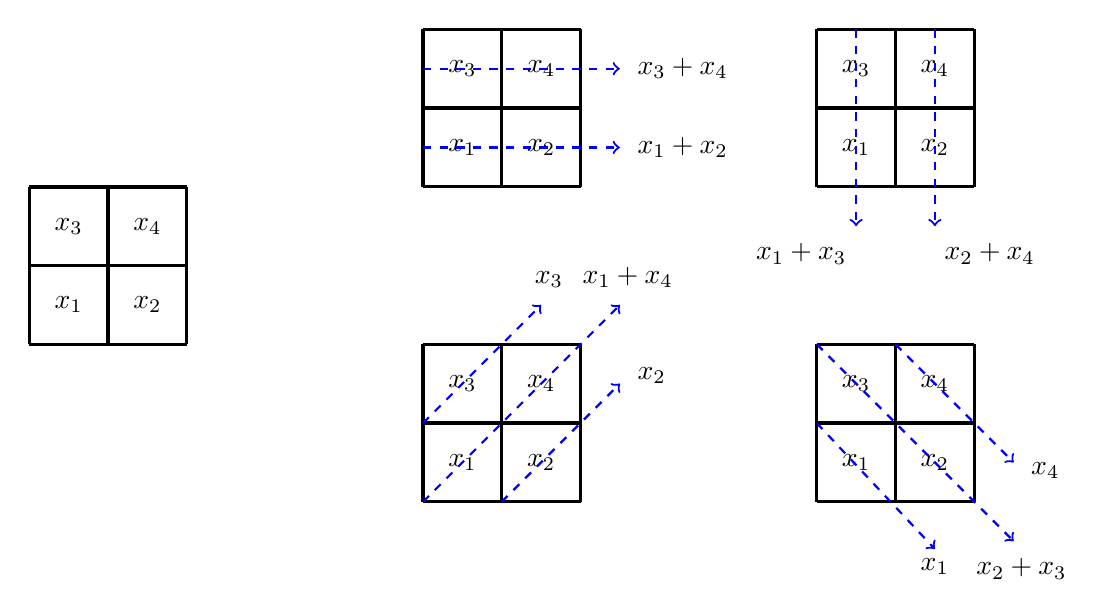
\begin{tikzpicture}[scale=1.0]
  \begin{scope}[yshift=-2cm]
    \draw[very thick] (0, 0) grid (2, 2);
    \node[anchor=center] at (0.5, 0.5) {\(x_1\)};
    \node[anchor=center] at (1.5, 0.5) {\(x_2\)};
    \node[anchor=center] at (0.5, 1.5) {\(x_3\)};
    \node[anchor=center] at (1.5, 1.5) {\(x_4\)};
  \end{scope}
  % horizontal measurements
  \begin{scope}[xshift=5cm]
    \draw[very thick] (0, 0) grid (2, 2);
    \node[anchor=center] at (0.5, 0.5) {\(x_1\)};
    \node[anchor=center] at (1.5, 0.5) {\(x_2\)};
    \node[anchor=center] at (0.5, 1.5) {\(x_3\)};
    \node[anchor=center] at (1.5, 1.5) {\(x_4\)};
    %
    \draw[thick,blue,dashed,->] (0.0,0.5) -- (2.5,0.5);
    \node[anchor=west] at (2.6,0.5) {\(x_1+x_2\)};
    \draw[thick,blue,dashed,->] (0.0,1.5) -- (2.5,1.5);
    \node[anchor=west] at (2.6,1.5) {\(x_3+x_4\)};
  \end{scope}
  % vertical measurements
  \begin{scope}[xshift=10cm]
    \draw[very thick] (0, 0) grid (2, 2);
    \node[anchor=center] at (0.5, 0.5) {\(x_1\)};
    \node[anchor=center] at (1.5, 0.5) {\(x_2\)};
    \node[anchor=center] at (0.5, 1.5) {\(x_3\)};
    \node[anchor=center] at (1.5, 1.5) {\(x_4\)};
    %
    \draw[thick,blue,dashed,->] (0.5,2.0) -- (0.5,-0.5);
    \node[anchor=north east] at (0.5,-0.6) {\(x_1+x_3\)};
    \draw[thick,blue,dashed,->] (1.5,2.0) -- (1.5,-0.5);
    \node[anchor=north west] at (1.5,-0.6) {\(x_2+x_4\)};
  \end{scope}
  % diagonal measurements
  \begin{scope}[xshift=5cm,yshift=-4cm]
    \draw[very thick] (0, 0) grid (2, 2);
    \node[anchor=center] at (0.5, 0.5) {\(x_1\)};
    \node[anchor=center] at (1.5, 0.5) {\(x_2\)};
    \node[anchor=center] at (0.5, 1.5) {\(x_3\)};
    \node[anchor=center] at (1.5, 1.5) {\(x_4\)};
    %
    \draw[thick,blue,dashed,->] (0.0,0.0) -- (2.5,2.5);
    \node[anchor=south] at (2.6,2.6) {\(x_1+x_4\)};
    \draw[thick,blue,dashed,->] (1.0,0.0) -- (2.5,1.5);
    \node[anchor=west] at (2.6,1.6) {\(x_2\)};
    \draw[thick,blue,dashed,->] (0.0,1.0) -- (1.5,2.5);
    \node[anchor=south] at (1.6,2.6) {\(x_3\)};
  \end{scope}
  % diagonal measurements
  \begin{scope}[xshift=10cm,yshift=-4cm]
    \draw[very thick] (0, 0) grid (2, 2);
    \node[anchor=center] at (0.5, 0.5) {\(x_1\)};
    \node[anchor=center] at (1.5, 0.5) {\(x_2\)};
    \node[anchor=center] at (0.5, 1.5) {\(x_3\)};
    \node[anchor=center] at (1.5, 1.5) {\(x_4\)};
    %
    \draw[thick,blue,dashed,->] (0.0,2.0) -- (2.5,-0.5);
    \node[anchor=north] at (2.6,-0.6) {\(x_2+x_3\)};
    \draw[thick,blue,dashed,->] (0.0,1.0) -- (1.5,-0.6);
    \node[anchor=north] at (1.5,-0.6) {\(x_1\)};
    \draw[thick,blue,dashed,->] (1.0,2.0) -- (2.5,0.5);
    \node[anchor=west] at (2.6,0.4) {\(x_4\)};
  \end{scope}
\end{tikzpicture}
\caption{Our CT model with four ``X-ray pictures'' of a \(2\times 2\)
object \([x_1,x_2,x_3,x_4]\in \mathbb{R}^4\) from four angles.
In this model we measure (assuming that the measurements do not contain errors) a vector \(b=[x_1+x_2,x_3+x_4,x_1+x_3,x_2+x_4,x_2,x_1+x_4,x_3,x_1,x_2+x_3,x_4]\in \mathbb{R}^{10}\).
In reality, typically we will measure a vector \(\tilde{b}=b+f \in \mathbb{R}^{10}\), where
\(f\in \mathbb{R}^{10}\) is a vector with unknown/random measurement errors.}\label{CT1}
\end{figure}

\begin{enumerate}
  \item Based on the description in Fig.~\ref{CT1}, find the matrix
  \(A\) representing our measurement model.
  That is, find \(A\), such that the CT problem to determine \(x=[x_1,x_2,x_3,x_4]\) from the measurements (without errors) reduces to solving a linear system \(Ax=b\).
  What is the size of \(A\)?
  \item[\textbf{Answer}] 
  \begin{align*}
    Ax=b \Longleftrightarrow A\begin{bmatrix}x_1 \\ x_2 \\ x_3 \\x_4 \end{bmatrix}=\begin{bmatrix}
    x_1+x_2 \\ x_3+x_4 \\ x_1 + x_3 \\ x_2 + x_4 \\ x_2 \\ x_1 + x_4 \\ x_3 \\ x_1 \\ x_2 + x_3 \\ x_4
    \end{bmatrix}
      \Longleftrightarrow 
    \begin{bmatrix}
    1 & 1 & 0 & 0 \\
    0 & 0 & 1 & 1 \\
    1 & 0 & 1 & 0 \\
    0 & 1 & 0 & 1 \\
    0 & 1 & 0 & 0 \\
    1 & 0 & 0 & 1 \\
    0 & 0 & 1 & 0 \\
    1 & 0 & 0 & 0 \\
    0 & 1 & 1 & 0 \\
    0 & 0 & 0 & 1 \\
    \end{bmatrix}
    \begin{bmatrix}x_1 \\ x_2 \\ x_3 \\x_4 \end{bmatrix}=\begin{bmatrix}
    x_1+x_2 \\ x_3+x_4 \\ x_1 + x_3 \\ x_2 + x_4 \\ x_2 \\ x_1 + x_4 \\ x_3 \\ x_1 \\ x_2 + x_3 \\ x_4
    \end{bmatrix}
  \end{align*}
  $A=n \times m$, $x=m \times p$ then $b=n \times p$ \\
  The size of $A$ must be $\mathbf{10 \times 4}$ matrix because if $A=10 \times 4$ and $x=4 \times 1$ then $b=10 \times 1$.

  \item Assuming now that the measurements contain unknown errors, i.e., that instead of the exact vector \(b\) we measure a different vector
  \(\tilde{b} = b + f\).
  Explain why the system \(Ax=\tilde{b}\) may lack solutions.
  Explain the concept ``least squares problem'' for such systems of linear algebraic equations.
  \item[\textbf{Answer}] When there is noise in the solution, it may become inconsistent (not solvable), as the measured value is no longer just dependent on the pixels it passes through. It therefore becomes the matter of solving the least squares problem, which finds the best approximate solution, by solving for the $x$ where $Ax$ gives the minimum difference to $b$. Hence finding the sum where $b-Ax$ is minimized.

  \item Let us now look at an object consisting of \(N\times N\) grayscale pixels, where \(N\geq 2\).
  Assuming that we still only take \(4\) X-ray pictures as in Fig.~\ref{CT1},
  what are the dimensions of \(x\), \(b\), and \(A\) in this situation?
  \item[\textbf{Answer}] 
  \begin{align*}
    A=6N-2\times N^2 \\
    x=N^2 \times 1 \\
    b=6N-2 \times 1
  \end{align*}

  \item Continuing as in the previous question with a \(N\times N\) object,
  utilize Theorem 8 from Section 1.7 in [Lay] to determine, for which
  \(N \geq 2\) the columns in the matrix \(A\) are necessarily \emph{linearly dependent}?
  \item[\textbf{Answer}]
  \textbf{Definition:} If a set contains more vectors than there are entries in each vector, then the set is linearly dependent. That is, any set $\{\mathbf{v}_1, . . . , \mathbf{v}_p\}$ in $\mathbb{R}^n$ is linearly dependent if $p > n$. \\
  We can insert $6n-1$ and $n^2$ into a graph and check for which values $N^2>6N-2$.

  \def\FunctionF(#1){(#1)^2}
  \def\FunctionG(#1){6*(#1)-2}

  \begin{align*}
    \begin{tikzpicture}
      \begin{axis}[
            axis y line=center,
            axis x line=middle, 
            axis on top=true,
            xmin=-1,
            xmax=8,
            ymin=-8,
            ymax=50,
            height=8.0cm,
            width=12.0cm,
            grid,
            xtick={-2,...,8},
            ytick={-5,0,...,50},
        ]
        \addplot [domain=2:50, samples=50, mark=none, ultra thick, blue] {\FunctionF(x)};
        \addplot [domain=2:50, samples=50, mark=none, ultra thick, red] {\FunctionG(x)};
        \addplot [domain=-20:2, dotted, samples=50, mark=none, ultra thick, blue] {\FunctionF(x)};
        \addplot [domain=-20:2, dotted, samples=50, mark=none, ultra thick, red] {\FunctionG(x)};
        \node [right, blue] at (axis cs: 2,45) {$N^2$};
        \node [right, red] at (axis cs: 2,40) {$6N-2$};
        \filldraw[blue] (5.64,31.87) circle (2pt) node[anchor=east,text=black]{(5.64,31.87)};
        %\filldraw[blue] (2,0) circle (2pt) node[anchor=south,text=black]{(2.0)};
        %\filldraw[blue] (3,12) circle (2pt) node[anchor=west,text=black]{(3,12)};
      \end{axis}
    \end{tikzpicture}
  \end{align*}

  We can see on the graph that if $N \geq 5.64$, then the columns in the matrix $A$ are necessarily linearly dependent because $N^2>6N-2$ whenever $N > 5.64$. This means that $A$ has more columns than entries whenever $N>5.64$ and is therefore linearly for $N>5.64$.

  \begin{align*}
    n^2-6n+2=0 \\
    n_1=\frac{6+\sqrt{6^2-4*1*2}}{2*1}=5.64 \\
    n_2=\frac{6-\sqrt{6^2-4*1*2}}{2*1}=0.35
  \end{align*}

  We choose $n_1$ because $n \geq 2$.

  \item Explain how QR-factorization of a matrix \(A\) can be used to solve a least-squares problem \(\min_{x} \|Ax-b\|^2\).
  \item[\textbf{Answer}] QR-factorization of a matrix allows expressing a matrix $A$ as the product of two matrices $Q$ and $R$. $Q$ is an orthogonal matrix with orthonormal basises and $R$ is an upper triangular matrix.
  \begin{align*}
    Ax=b \\ A^TAx=A^Tb \\ (QR)^T(QR)x=(QR)^Tb \\ R^TQ^TQRx=R^TQ^Tb \\
    R^TR=Q^TR^Tb \\
    R=Q^Tb
  \end{align*}
  We can see that $x$ can be solved my matrix multiplication $R=Q^Tb$, and this is only possible if the columns of $A$ are linearly independent.

  \item On moodle there are Python and Matlab scripts, illustrating how a QR factorization of a given matrix can be computed.\footnote{They also illustrate, how to multiply matrices.  To solve a system of linear algebraic equations, use ``numpy.linalg.solve'' in Python or ``backslash'' operator in Matlab.}
  Compute a QR-factorization of the matrix \(A\) associated with our simplified CT measurement model for a \(N\times N\) object with \(N=2\).
  Furthermore, using this information  compute the orthogonal projection of the vector \(b = [0,1,2,3,4,5,6,7,8,9]\in \mathbb{R}^{10}\) onto the linear subspace spanned by the columns of \(A\) (recall that  \(\text{col}(A) = \text{col}(Q)\)).
  \item[\textbf{Answer}] By using MATLAB the orthogonal basis of the vector $b$ is calculated as follows: \\
  We start by finding $Q$ and $R$ by using MATLAB.
  \begin{align*}
	Q=\begin{bmatrix}
    	-0.5000 & -0.3873 & 0.2108 & 0.1782 \\
		0 & 0 & -0.5270 & -0.4454 \\
		-0.5000 & 0.1291 & -0.4216 & 0.1782 \\
		0 & -0.5164 & 0.1054 & -0.4454 \\
		0 & -0.5164 & 0.1054 & 0.0891 \\
		-0.5000 & 0.1291 & 0.1054 & -0.4454 \\
		0 & 0 & -0.5270 & 0.0891 \\
		-0.5000 & 0.1291 & 0.1054 & 0.0891 \\
		0 & -0.5164 & -0.4216 & 0.1782 \\
		0 & 0 & 0 & -0.5345
    \end{bmatrix} \\
    R=\begin{bmatrix}
    	-2 & -0.5 & -0.5 & -0.5 \\
		0 & -1.9365 & -0.3873 & -0.3873 \\
		0 & 0 & -1.8974 & -0.3162 \\
		0 & 0 & 0 & -1.8708
    \end{bmatrix} \\
   \end{align*}
   We now have an orthonormal basis $Q$ and the upper triangular matrix $R$ by definition of QR-factorization. By using the formula $Q(Q^T\mathbf{b})$ we can compute the projection:
   \begin{align*}
	proj_Qb=\begin{bmatrix}
      3.5714 \\
      5.5714 \\
      4.2381 \\
      4.9048 \\
      1.9524 \\
      4.5714 \\
      2.6190 \\
      1.6190 \\
      4.5714 \\
      2.9524
    \end{bmatrix}
  \end{align*}

  \item Find the solution to the least-squares problem associated with our simplified CT model for a \(N\times N\) object with \(N=2\) corresponding to the measurements \(b = [0,1,2,3,4,5,6,7,8,9]\in \mathbb{R}^{10}\).
  Use two alternative methods: solving the normal equations and utilizing the QR-factorization.
  \item[\textbf{Answer}] 
  Method 1 (normal equations):
  \begin{align*}
    \mathbf{\hat{x}} \Longleftrightarrow A^TA\mathbf{x}=A^T\mathbf{b} \Longleftrightarrow
    \begin{bmatrix}
      1.6190 \\ 1.9524 \\ 2.6190 \\ 2.9524
    \end{bmatrix}
  \end{align*}
  Method 2 (Utilizing QR-factorization):
  \begin{align*}
    \mathbf{\hat{x}} \Longleftrightarrow R\mathbf{x}=Q^T\mathbf{b}\begin{bmatrix}
      1.6190 \\ 1.9524 \\ 2.6190 \\ 2.9524
    \end{bmatrix}
  \end{align*}
\end{enumerate}

\section*{Part 2: QR-factorization using Given's rotations}

Consider a nonzero vector \([a,b] \in \mathbb{R}^2\).
Given's rotation is an orthogonal transformation (as the name suggests, a rotation) which maps \([a,b]\) to a vector \([d,0]\in \mathbb{R}^2\)
aligned with the first coordinate axis.

\begin{enumerate}
  \item Use Theorem 7 in Subsection 6.2 [Lay], to determine \(|d|\)
  given \([a,b]\).
  \item[\textbf{Answer}] 
  \begin{align*}
    ||Ux|| = \begin{bmatrix}
      a \\ b
    \end{bmatrix}
    \begin{bmatrix}
      x
    \end{bmatrix}
    =
    \begin{bmatrix}
      ax \\ bx
    \end{bmatrix}
    =
    \begin{bmatrix}
      ax-bx \\ 0
    \end{bmatrix}
    =
    \sqrt{(ax-bx)^2+0^2}
    =
    \sqrt{d^2+0^2}
    =
    ||d||
  \end{align*}

  \item Verify that
  \begin{equation}\label{eq:givens}
    G = \begin{bmatrix}
    c & s\\-s&c
  \end{bmatrix},
\end{equation}
  where \(c = a/\sqrt{a^2 + b^2}\) and \(s = b/\sqrt{a^2 + b^2}\)
  is a Given's rotation.
  That is, check that \(G\) is an orthogonal matrix that maps \([a,b]\) to \([d,0]\).
  \item[\textbf{Answer}] 
  To check if the $G$ is a orthogonal matrix we can check that $G^TG=I$ is true.
  \begin{align*}
    G^TG=
    \begin{bmatrix}
      c & -s \\ s & c
    \end{bmatrix}
    \begin{bmatrix}
      c & s \\ -s & c
    \end{bmatrix}
    =
    \begin{bmatrix}
      cc+ss & cs-sc \\ sc-cs & ss+cc
    \end{bmatrix}
    =
    \begin{bmatrix}
      cc+ss & 0 \\ 0 & ss+cc
    \end{bmatrix}
    =
    \begin{bmatrix}
      1 & 0 \\ 0 & 1
    \end{bmatrix}
  \end{align*}
  $G^TG=I$ is in fact true, therefore $G$ is a orthogonal matrix. Now we can check if $G$ maps $[a,b]$ to $[d,0]$
  \begin{multline*}
    \begin{bmatrix}
      c & s \\ -s & c
    \end{bmatrix}
    \begin{bmatrix}
      a \\ b
    \end{bmatrix}
    =
    \begin{bmatrix}
      a/\sqrt{a^2+b^2} & b/\sqrt{a^2+b^2} \\ -(b/\sqrt{a^2+b^2}) & a/\sqrt{a^2+b^2}
    \end{bmatrix}
    \begin{bmatrix}
      a \\ b
    \end{bmatrix}
    =
    \begin{bmatrix}
      a/\sqrt{a^2+b^2} * a + b/\sqrt{a^2+b^2} * b \\ -(b/\sqrt{a^2+b^2}) * a + a/\sqrt{a^2+b^2} * b
    \end{bmatrix} \\
    =
    \begin{bmatrix}
      a^2/\sqrt{a^2+b^2} + b^2/\sqrt{a^2+b^2} \\ 0
    \end{bmatrix}
  \end{multline*}
  We can see that in fact, $G$ does map $[a,b]$ to a vector $[d,0]$ in $\mathbb{R}^2$.
  \item Let us now consider a vector \(x \in \mathbb{R}^m\),
  \(m\geq 2\), such that \(x_i = a\) and \(x_j = b\), \(i<j\).
  We compute \(c\) and \(s\) as in the previous question.
  Let now \(G(i,j,a,b)\) be an \(m\times m\) matrix, with all
  rows/columns as in the identity matrix, with the exception of the rows/columns \(i\) and \(j\), where we ``insert'' the
  matrix \(G\) from~\eqref{eq:givens}, i.e.:
  \(G(i,j,a,b)_{ii}=G(i,j,a,b)_{jj}=c\),
  \(G(i,j,a,b)_{ij}=-G(i,j,a,b)_{ji}=s\):
  \begin{equation}\label{eq:givens2}
    G(i,j,a,b)=\begin{bmatrix}
    I\\
    & c & & s \\
    &   &I&   \\
    & -s && c \\
    &&&&I
  \end{bmatrix}.
  \end{equation}
  Verify that \(G(i,j,a,b)\) is an orthogonal matrix, and that
  \begin{equation}\label{eq:givens1}
  G(i,j,a,b) x = \begin{bmatrix}
  x_1 \\ \vdots \\ x_{i-1}\\ d \\ x_{i+1}\\\vdots\\x_{j-1}\\0\\x_{j+1}\\\vdots\\x_{m}
  \end{bmatrix}
  \end{equation}
  \item[\textbf{Answer}]
  \begin{align*}
      GG^T=
      \begin{bmatrix}
        I\\
        & c & & s \\
        &   &I&   \\
        & -s && c \\
        &&&&I
      \end{bmatrix}
      \begin{bmatrix}
        I\\
        & c & & -s \\
        &   &I&   \\
        & s && c \\
        &&&&I
      \end{bmatrix}
      =
      \begin{bmatrix}
        I\\
        & cc+ss & & sc-sc \\
        &   &I&   \\
        & sc-cs && ss+cc \\
        &&&&I
      \end{bmatrix}
      =
      \begin{bmatrix}
        I\\
        & 1 \\
        &   &I&   \\
        & && 1 \\
        &&&&I
      \end{bmatrix} \\
      G(2,4,a,b)x=
      \begin{bmatrix}
        I\\
        & c & & s \\
        &   &I&   \\
        & -s && c \\
        &&&&I
      \end{bmatrix}
      \begin{bmatrix}
        x_1 \\ a \\ x_3 \\ b \\ x_5
      \end{bmatrix}=
      \begin{bmatrix}
        x_1 \\
        ca+sb \\
        x_3 \\
        -sa+cb \\
        x_5
      \end{bmatrix}
      =
      \begin{bmatrix}
        x_1 \\
        ca+sb \\
        x_3 \\
        -(b/\sqrt{a^2+b^2})a+(a/\sqrt{a^2+b^2})b \\
        x_5
      \end{bmatrix}
      =
      \begin{bmatrix}
        x_1 \\
        d \\
        x_3 \\
        0 \\
        x_5
      \end{bmatrix}
  \end{align*}
  \begin{align*}
    G(i,j,a,b)x=
    \begin{bmatrix}
      I\\
      & \ddots \\
      && c_{ii} & & s_{ij} \\
      &&    &I&   \\
      && -s_{ji} && c_{jj} \\
      &&&&& \ddots \\
      &&&&&& I
    \end{bmatrix}
    \begin{bmatrix}
      x_1 \\ \vdots \\ x_{i-1} \\ a \\ x_{i+1} \\ \vdots \\ x_{j-1} \\ b \\ x_{j+1} \\ \vdots \\ x_m
    \end{bmatrix}
  \end{align*}
  For all $x_1 \ldots x_{i-1}, x_{i+1} \ldots x_{j-1}$ and $x_{j+1} \ldots x_m$ the corresponding rows in $G$ are the identity matrix which means the values will match the original $x$ value.
  
  For $x_i$ the value will be the row $i$ of $G$ multiplied by $x$. Since the only non-zero values in the row $i$ of $G$ is $c$ and $s$ the value will equal:
  \begin{align*}
  	cx_i+sx_j=ca+sb=a \frac{a}{\sqrt{a^2+b^2}}+b\frac{b}{\sqrt{a^2+b^2}}=\frac{a^2}{\sqrt{a^2+b^2}}+\frac{b^2}{\sqrt{a^2+b^2}}=\frac{a^2+b^2}{\sqrt{a^2+b^2}}=d
  \end{align*}
  For $x_j$ the value will be the row $j$ of $G$ multiplied by $x$. Since the only non-zero values in the row $j$ of $G$ is $-s$ and $c$, the values will equal:
  \begin{align*}
  	-sx_i+cx_j=-sa+cb=-a\frac{b}{\sqrt{a^2+b^2}}+b\frac{a}{\sqrt{a^2+b^2}}=\frac{-ab}{\sqrt{a^2+b^2}}+\frac{ab}{\sqrt{a^2+b^2}}=\frac{-ab+ab}{\sqrt{a^2+b^2}}=0
  \end{align*}

  \item Explain why a product of square orthogonal matrices is itself an orthogonal matrix.
  I.e., assuming that \(Q_1, Q_2,\dots, Q_k\) are orthogonal matrices, explain why the matrix \(Q_1 Q_2 \cdots Q_k\) is orthogonal.
  \item[\textbf{Answer}]
  Let $A$ and $B$ be orthogonal matrices.
  \begin{align*}
    AA^T=A^TA=I
  \end{align*}
  and
  \begin{align*}
    BB^T=B^TB=I
  \end{align*}
  Then we have a new vector $AB$. An matrix is a orthogonal matrix if $G^TG=I$ is true. Let's try to do that by replacing $G$ with our new vector $AB$ and check if we make it equal the identity matrix.
  \begin{align*}
    (AB)^T(AB)=(B^TA^T)AB=\mathbf{B^T(A^TA)B}=B^T(I)B=B^TB=I
  \end{align*}
  The equation highlighted in \textbf{BOLD} are using the matrix property $(AB)C=A(BC)$.

  We can see that the product of two orthogonal matrices is a new orthorgnal matrix because the rule $G^TG=I$ is true. Hence we get a new orthogonal matrix. Since they are all orthogonal matrices, the matrix $Q_1 Q_2 \cdots Q_k$ is orthogonal.

  \item Consider the following algorithm, where the matrix \(A\) of size \(m\times n\) is given.
  \begin{algorithmic}
    \STATE \(Q:= I_{m\times m}\); \(R:= A\);
    \FOR {\(i=1,\dots,n\)}
    \FOR {\(j=i+1,\dots,m\)}
    \STATE \(a = R_{ii}\); \(b = R_{ji}\);
    \IF {\(b \neq 0\)}
    \STATE \(R := G(i,j,a,b)R\); \(Q := Q G(i,j,a,b)^T\);
    \ENDIF
    \ENDFOR
    \ENDFOR
  \end{algorithmic}
  where \(G(i,j,a,b)\) is given by~\eqref{eq:givens2}.
  \begin{enumerate}
    \item Use the previous questions to explain, why the matrix \(Q\) remains orthogonal throughout all iterations of the algorithm.
    \item[\textbf{Answer}] We just saw from question 3, that $G(i,j,a,b)$ is an orthogonal matrix. The identify matrix ($I$) is also an orthogonal matrix. Because the next $Q$ in the loop is equal to $QG(g,i,a,b)^T$. That is, an orthogonal matrix times an orthogonal matrix which we from question 4 found to equal a new orthogonal matrix. Hence it will reamin orthogonal thorugh all iterations.
    \item Explain why the equation \(A=QR\) is fullfilled throughout all iterations of the algorithm.
    \item[\textbf{Answer}] Initially, the $Q=I$ and $R=Q$, therefore $A=QR$. Throughout the loop we get that $R=G(i,j,a,b)R$ and $Q=QG(i,j,a,b)^T$, hence we get
    \begin{align*}
      A=(QG(i,j,a,b)^T)(G(i,j,a,b)R)=Q(G(i,j,a,b)^TG(i,j,a,b))R=Q(I)R=QR
    \end{align*}
    We can see that the equation will remain $A=QR$ throughout all iterations of the alogithm.
    \item Use~\eqref{eq:givens1} to explain, why after the algorithm terminates, the computed matrix \(R\) is upper triangular.
    \item[\textbf{Answer}] We saw in question~\eqref{eq:givens1}, that the element at index $x_j$ will equal zero when multiplied by a column vector ($m \times 1$). The outer \textbf{for} loop iterates through the columns and the inner \textbf{for} loop iterates through the rows beginning at column $i+1$ up to $m$. It updates $R$ to equal $G(i,j,a,b)R$ which sets the element at $x_{ji}$ to equal 0. The entries below the diagonal will therefore all equal 0 making $R$ an upper triangular matrix.
  \end{enumerate}
\end{enumerate}

\end{document}
